\begin{exercise}{2016/17 2}
    \emph{Το σύστημα του \tl{Duffing}}: Το σύστημα
    \begin{align*}
        \dot{x} &= y \\
        \dot{y} &= -\zeta y + x - x^3, \quad \zeta \geq 0
    \end{align*}
    στο επίπεδο είναι η κανονική μορφή της αυτόνομης Δ.Ε.
    \begin{equation*}
        \ddot{x} + \zeta\dot{x} + x^3 - x = 0.
    \end{equation*}
    περιγράφει ένα σύστημα με απόσβεση που κινείται σε συμμετρικό δυναμικό με
    δύο ελάχιστα (γιατί;)
    \begin{enumerate}[label = (\alph*)]
        \item Θα μελετήσουμε πρώτα την περίπτωση \( \zeta = 0 \). Το σύστημα
            είναι συντηρητικό (Χαμιλτονιανό), της μορφής \( \dot{x} = y, \dot{y}
            = - \nabla U(x) \). Επαληθεύστε ότι ισχύει αυτό, δώστε την
            Χαμιλτονιανή συνάρτηση \( H(x, y) \) και το διάγραμμα ροής (πορτρέτο
            κίνησης ή φάσεων).
        \item Τώρα περνάμε στην περίπτωση \( \zeta > 0 \). Βρείτε τα σημεία
            ισορροπίας και την (τοπική) τους συμπεριφορά. Δείξτε ότι, κατάλληλα
            μετατοπισμένη, η \( H \) είναι συνάρτηση \tl{Lyapunov} και εξηγήστε
            γιατί αποτελεί υποσύνολο της περιοχής έλξης κάθε Σ.Ι. Δείξτε ότι εάν
            \emph{τρέξουμε} τα σύνολα αυτά προς τα πίσω (σε αρνητικό χρόνο) θα
            πάρουμε τη συνολική έλξης. Προσπαθήστε να δώσετε ένα διάγραμμα των
            περιοχών αυτών για διάφορες τιμές του \( \zeta \). Πόσες
            καμπύλες/τροχιές αποτελούν το διαχωριστικό σύνολο των δύο περιοχών
            έλξης;
    \end{enumerate}
\end{exercise}
\begin{solution}{2016/17 2}
    1. Οι εξισώσεις του συστήματος χωρίς απόσβεση είναι
    \begin{align*}
        \dot{x} &= y \\
        \dot{y} &= x - x^3.
    \end{align*}
    Τα σημεία ισορροπίας υπολογίζονται από τις σχέσεις
    \begin{align*}
        0 &= y \\
        0 &= x - x^3,
    \end{align*}
    και από τη δεύτερη σχέση έχουμε
    \begin{equation*}
        x(1 - x^2) = 0,
    \end{equation*}
    που σημαίνει \( x = 0 \) ή \( x = \pm 1 \). Άρα έχουμε τα σημεία
    ισορροπίας είναι \( (0, 0), (1, 0), (-1, 0) \).

    Επειδή δεν έχουμε απόσβεση, έχουμε Χαμιλτονιανό δυναμικό σύστημα με
    \( q = x, p = y \) και θέλουμε
    \begin{equation*}
        \frac{\partial H}{\partial y} = y, \quad
        \frac{\partial H}{\partial x} = -x + x^3.
    \end{equation*}
    Έτσι θέλουμε
    \begin{equation}\label{eq:ex2_hamiltonian}
        H(x, y) = \frac{1}{2}y^2 + U(x),
    \end{equation}
    με συνάρτηση δυναμικού
    \begin{align}\label{eq:ex2_potential}
        U(x) &= - \int_0^x \left(\bar{x} - \bar{x}^3 \right) \, d\bar{x}
        \nonumber \\
        &= -\frac{1}{2}x^2 + \frac{1}{4}x^4.
    \end{align}
    Μάλιστα μπορούμε να επιβεβαιώσουμε ότι είναι Χαμιλτονιανό καθώς έχουμε
    \begin{align*}
        \frac{dH}{dt}
        &= y\dot{y} - x\dot{x} + x^3\dot{x} \\
        &= y(x - x^3) - xy + x^3y = 0.
    \end{align*}
    Συνεπώς, το σύστημα είναι της μορφής
    \begin{align*}
        \dot{x} &= y \\
        \dot{y} &= -\nabla U(x) = -\nabla\left( -\frac{1}{2}x^2 +
        \frac{1}{4}x^4 \right),
    \end{align*}
    ή τελικά
    \begin{align*}
        \dot{x} &= y \\
        \dot{y} &= x - x^3.
    \end{align*}
    Από τη σχέση~\eqref{eq:ex2_hamiltonian}, διαπιστώνουμε ότι οι λύσεις του
    συστήματος, είναι συμμετρικές ως προς τον άξονα των τετμημένων, καθώς
    η συνολική ενέργεια \( H(x, y) \) είναι σταθερή. Έτσι κάθε λύση ή τροχιά
    ανήκει σε μία ισοϋψή καμπύλη που εξαρτάται από την αρχική ενέργεια
    \( h_0 \). Έτσι οι λύσεις είναι
    \begin{equation*}
        y = \pm \sqrt{2h_0 + x^2 - \frac{1}{2}x^4}.
    \end{equation*}
    Η κλίση των τροχιών στο επίπεδο φάσεων είναι
    \begin{equation*}
        \frac{dy}{dx} = \frac{x - x^3}{y}.
    \end{equation*}
    Από τη σχέση της συνάρτησης δυναμικού~\eqref{eq:ex2_potential} καθώς από
    την παραπάνω σχέση φαίνεται ότι η συνάρτηση δυναμικού παρουσιάζει ακρότατο
    στα σημεία ισορροπίας. Αυτό συμβαίνει διότι εκεί ισχύει
    \begin{align*}
        0 &= U'(x) \\
        &= x^3 - x,
    \end{align*}
    και έτσι επιβεβαιώνεται ότι τα κρίσιμα σημεία της συνάρτησης είναι τα
    \( 0, \pm 1 \).

    Για να χαρακτηρίσουμε τα σημεία ισορροπίας, γράφουμε τις εξισώσεις που
    διέπουν το σύστημα στη μορφή
    \begin{equation*}
        \begin{pmatrix}
            \dot{x} \\
            \dot{y}
        \end{pmatrix} = F(x, y) =
        \begin{pmatrix}
            y \\
            x - x^3
        \end{pmatrix}.
    \end{equation*}
    Αν πάρουμε τη γραμμικοποίηση, θα έχουμε
    \begin{equation*}
        DF(x, y) =
        \begin{pmatrix}
            0 & 1 \\
            1 - 3x^2 & 0
        \end{pmatrix}.
    \end{equation*}

    Για το σημείο ισορροπίας \( (0, 0) \) ισχύει
    \begin{equation*}
        DF(0, 0) =
        \begin{pmatrix}
            0 & 1 \\
            1 & 0
        \end{pmatrix}
    \end{equation*}
    που συνεπάγεται
    \begin{equation*}
        \lambda_1 = 1, \quad \lambda_2 = -1.
    \end{equation*}
    Από το θεώρημα \tl{Hartman–Grobman}, επειδή το σημείο είναι
    υπερβολικό, και επειδή έχουμε σάγμα στο \( (0, 0) \) στο γραμμικοποιημένο
    σύστημα, θα έχουμε σάγμα στο \( (0, 0) \) και για το αρχικό μη-γραμμικό
    σύστημα.

    Με αντίστοιχη διαδικασία, για το σημείο ισορροπίας \( (1, 0) \) ισχύει
    \begin{equation*}
        DF(1, 0) =
        \begin{pmatrix}
            0 & 1 \\
            -2 & 0
        \end{pmatrix}
    \end{equation*}
    που συνεπάγεται
    \begin{equation*}
        \lambda = \pm i\sqrt{2}.
    \end{equation*}
    Στην περίπτωση αυτή, έχουμε φανταστικές ιδιοτιμές και έτσι δεν μπορούμε να
    βγάλουμε κάποιο συμπέρασμα από το θεώρημα \tl{Hartman-Grobman}. Παρόλο αυτά
    έχουμε συμπεριφορά κέντρου στο \( (1, 0) \) για το γραμμικοποιημένο σύστημα.

    Στο ίδιο αποτέλεσμα καταλήγουμε και για το σημείο ισορροπίας \( (-1,
    0) \), καθώς ο όρος που σχετίζεται με τη μεταβλητή \(x\) στον πίνακα
    γραμμικοποίησης είναι τετραγωνικός.

    Η ακριβής φύση των κρίσιμων σημείων, μπορεί να καθοριστεί από τη συνάρτηση δυναμικού
    και από την τιμή της δεύτερης παραγώγου στα σημεία αυτά. Έτσι
    \begin{equation*}
        U''(x) = 3x^2 - 1.
    \end{equation*}
    Στα σημεία \( 1 \) και \( -1 \), η συνάρτηση δυναμικού παρουσιάζει τοπικό
    ελάχιστο, \( U''(1) = U''(-1) = 2 > 0 \), ενώ στο σάγμα \( U''(0) = -1 < 0
    \) τοπικό μέγιστο.

    \begin{figure}[h]
        \centering
        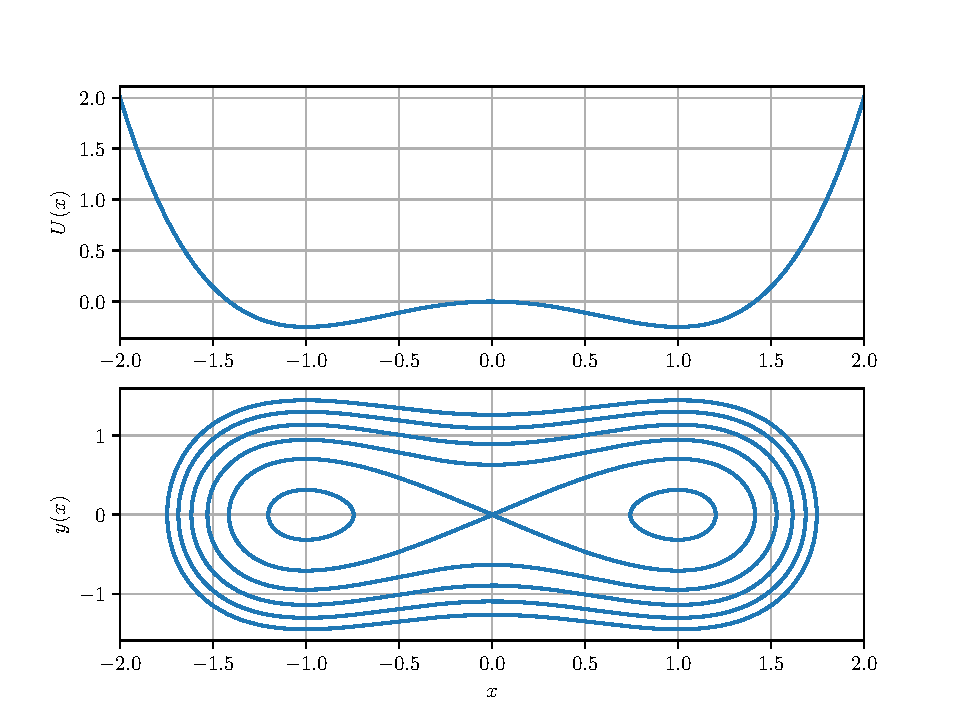
\includegraphics[width=0.9\textwidth]{figures/ex2_undampedDuffing.pdf}
        \caption{\gr{Συνάρτηση δυναμικού και ταλαντωτής \tl{Duffing} χωρίς απόσβεση.}}
        \label{fig:ex2_undampedDuffing}
    \end{figure}
    \begin{figure}[h]
        \centering
        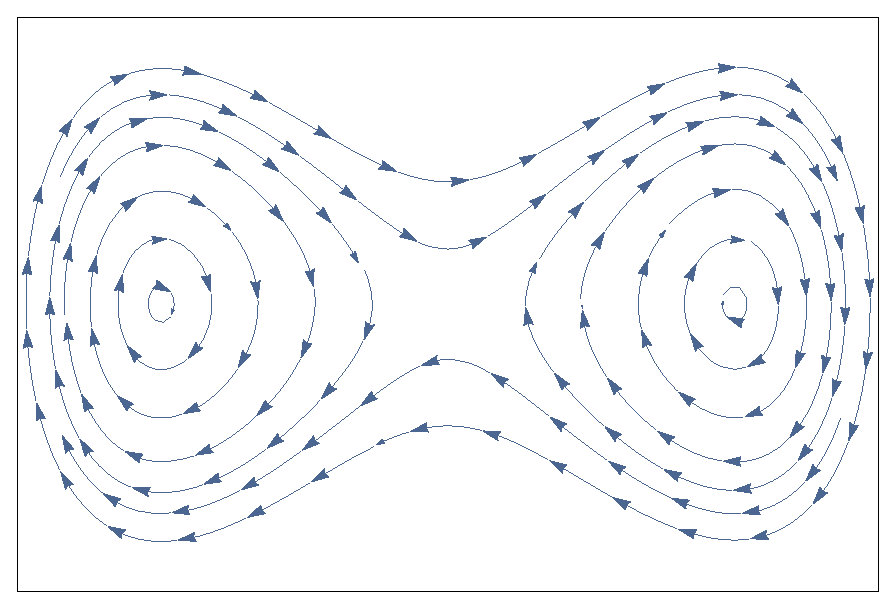
\includegraphics[width=0.8\textwidth]{figures/ex2_undampedDuffingVectorField.eps}
        \caption{\gr{Πορτρέτο κίνησης ταλαντωτή \tl{Duffing} χωρίς απόσβεση.}}
        \label{fig:ex2_undampedDuffingVectorField}
    \end{figure}
    Στο επάνω σχήμα της~\ref{fig:ex2_undampedDuffing} βλέπουμε τη συνάρτηση
    δυναμικού και στο κάτω το πορτρέτο φάσεων του ταλαντωτή \tl{Duffing} χωρίς
    απόσβεση. Όπως παρατηρούμε, η συνάρτηση δυναμικού παρουσιάζει τα ακρότατα
    στα σημεία ισορροπίας. Στα σημεία \( (-1, 0) \) και \( (1, 0) \) παρατηρούμε
    ότι έχουμε συμπεριφορά κέντρου, και στο σημείο \( (0, 0) \) έχουμε σάγμα.
    Στο σχήμα~\ref{fig:ex2_undampedDuffingVectorField} παρουσιάζεται η
    συμπεριφορά του διανυσματικού πεδίου.

    2. Στην περίπτωση όπου το \( \zeta > 0 \), οι εξισώσεις θα είναι
    \begin{equation*}
        \begin{pmatrix}
            \dot{x} \\
            \dot{y}
        \end{pmatrix} = F(x, y) =
        \begin{pmatrix}
            y \\
            -\zeta y + x - x^3
        \end{pmatrix}.
    \end{equation*}
    Τα σημεία ισορροπίας υπολογίζονται από τις σχέσεις
    \begin{align*}
        0 &= y \\
        0 &= -\zeta y + x - x^3,
    \end{align*}
    και από τη δεύτερη σχέση έχουμε
    \begin{equation*}
        x(1 - x^2) = 0,
    \end{equation*}
    που σημαίνει \( x = 0 \) ή \( x = \pm 1 \), και άρα έχουμε τα σημεία
    ισορροπίας παραμένουν τα ίδια και είναι \( (0, 0), (1, 0), (-1, 0) \).

    Η γραμμικοποίηση, είναι
    \begin{equation*}
        DF(x, y) =
        \begin{pmatrix}
            0 & 1 \\
            1 - 3x^2 & -\zeta
        \end{pmatrix}
    \end{equation*}
    και για το σημείο ισορροπίας \( (0, 0) \) ισχύει
    \begin{equation*}
        DF(0, 0) =
        \begin{pmatrix}
            0 & 1 \\
            1 & -\zeta
        \end{pmatrix}.
    \end{equation*}
    Οι ιδιοτιμές της γραμμικοποίησης στο \( (0, 0) \) είναι
    \begin{equation*}
        \det
        \begin{pmatrix}
            -\lambda & 1 \\
            1 & -\zeta - \lambda
        \end{pmatrix}.
    \end{equation*}
    που σημαίνει ότι
    \begin{equation*}
        \lambda^2 + \zeta \lambda - 1 = 0,
    \end{equation*}
    και μας δίνει τις λύσεις
    \begin{equation*}
        \lambda = \frac{1}{2}\left( -\zeta \pm \sqrt{\zeta^2 + 4} \right).
    \end{equation*}
    Αν συμβολίσουμε με \( \lambda_1 \) την ιδιοτιμή που προκύπτει από το θετικό
    πρόσημο που είναι μπροστά από την τετραγωνική ρίζα και αντίστοιχα με
    \( \lambda_2 \) την άλλη ιδιοτιμή, παρατηρούμε ότι \( \lambda_1 > 0 \).
    Γιατί αν ίσχυε \( \lambda_1 \leq 0 \) τότε
    \begin{align*}
        -\zeta + \sqrt{\zeta^2 + 4} &\leq 0 \\
        \sqrt{\zeta^2 + 4} &\leq \zeta \\
        \zeta^2 + 4 &\leq \zeta^2,
    \end{align*}
    άτοπο. Επίσης, είναι ξεκάθαρο ότι \( \lambda_2 < 0 \) διότι \( \zeta > 0 \)
    και άρα έχουμε σάγμα για τη γραμμικοποίηση. Συνεπώς, από το θεώρημα
    \tl{Hartman–Grobman}, επειδή το σημείο είναι υπερβολικό, θα έχουμε σάγμα στο
    \( (0, 0) \) και για το αρχικό μη-γραμμικό σύστημα.

    Για το σημείο ισορροπίας \( (1, 0) \) ισχύει
    \begin{equation*}
        DF(1, 0) =
        \begin{pmatrix}
            0 & 1 \\
            -2 & -\zeta
        \end{pmatrix}.
    \end{equation*}
    Οι ιδιοτιμές της γραμμικοποίησης στο \( (1, 0) \) είναι
    \begin{equation*}
        \det
        \begin{pmatrix}
            -\lambda & 1 \\
            -2 & -\zeta - \lambda
        \end{pmatrix}.
    \end{equation*}
    που σημαίνει ότι
    \begin{equation*}
        \lambda^2 + \zeta \lambda + 2 = 0,
    \end{equation*}
    και μας δίνει τις λύσεις
    \begin{equation*}
        \lambda = \frac{1}{2}\left( -\zeta \pm \sqrt{\zeta^2 - 8} \right).
    \end{equation*}
    Συμβολίζουμε με \( \lambda_1 \) την ιδιοτιμή με προκύπτει από το θετικό
    πρόσημο που είναι μπροστά από την τετραγωνική ρίζα και αντίστοιχα με
    \( \lambda_2 \) την άλλη ιδιοτιμή. Οι ρίζες της διακρίνουσας είναι \(
    -2\sqrt{2} \) και \( 2\sqrt{2} \). Όμως η απόσβεση είναι αυστηρά θετική και
    έτσι η διακρίνουσα είναι αρνητική για \( \zeta \in (0, 2\sqrt{2}) \) και
    θετική για \( \zeta > 2\sqrt{2} \).

    Στην περίπτωση όπου το \( \zeta \in (0, 2\sqrt{2}) \) τότε επειδή
    το πραγματικό μέρος είναι πάντα αρνητικό, το σημείο ισορροπίας \( (1,
    0) \), από το θεώρημα \tl{Hartman-Grobman}, είναι ασυμπτωτικά ευσταθές
    και έχει τη μορφή ευσταθούς εστίας.

    Στην περίπτωση όπου το \( \zeta > 2\sqrt{2} \) τότε φυσικά η \( \lambda_2 =
    1/2 \left( -\zeta - \sqrt{\zeta^2 - 8} \right) < 0 \), αλλά και η \( \lambda_1 =
    1/2 \left( -\zeta +\sqrt{\zeta^2 - 8} \right) < 0 \). Γιατί αν \( \lambda_1
    \geq 0 \) τότε
    \begin{align*}
        -\zeta + \sqrt{\zeta^2 - 8} &\geq 0 \\
        \zeta^2 - 8 &\geq \zeta^2,
    \end{align*}
    άτοπο.

    Άρα στην περίπτωση όπου το \( \zeta > 2\sqrt{2} \) τότε το σημείο
    ισορροπίας \( (1, 0) \), από το θεώρημα \tl{Hartman-Grobman}, είναι
    ασυμπτωτικά ευσταθές και έχει τη μορφή ευσταθούς κόμβου.

    Τέλος, για \( \zeta = 2\sqrt{2} \) έχουμε διπλή ρίζα και στο σημείο
    ισορροπίας \( (1, 0) \), από το θεώρημα \tl{Hartman-Grobman}, έχουμε
    ασυμπτωτική ευστάθεια, αλλά τείνουμε στο σημείο ισορροπίας με διαφορετική
    μορφή σε σχέση με την προηγούμενη περίπτωση.

    Ακριβώς στα ίδια αποτελέσματα καταλήγουμε και για το σημείο ισορροπίας
    \( (-1, 0) \), καθώς ο όρος που σχετίζεται με τη μεταβλητή \(x\) στον πίνακα
    γραμμικοποίησης είναι τετραγωνικός.

    Άρα ανακεφαλαιώνοντας, για τα σημεία ισορροπίας \( (1, 0) \) και \( (-1, 0)
    \) για θετική απόσβεση θα έχουμε πάντα ασυμπτωτική ευστάθεια.

    Θεωρώ τη συνάρτηση
    \begin{equation}\label{eq:ex2_lyapynov}
        V(x, y) = \frac{1}{2}y^2 - \frac{1}{2}x^2 + \frac{1}{4}x^4 +
        \frac{1}{4},
    \end{equation}
    ως υποψήφια συνάρτηση \tl{Lyapunov}.

    Παρατηρούμε ότι στα ευσταθή σημεία ισορροπίας \( (\pm1, 0) \) ισχύει
    \begin{equation*}
        V(1, 0) =  V(-1, 0) = -\frac{1}{2} + \frac{1}{4} + \frac{1}{4} = 0.
    \end{equation*}
    Επίσης, βλέπουμε από τη σχέση~\eqref{eq:ex2_lyapynov}, ότι η συνάρτηση \( V \)
    μπορεί να γραφτεί
    \begin{equation*}
        V(x, y) = \frac{1}{2}y^2 - \left( \frac{1}{2}x^2 - \frac{1}{2} \right),
    \end{equation*}
    που σημαίνει ότι είναι θετική για κάθε \( (x, y) \neq (\pm1, 0) \). Ο ρυθμός
    μεταβολής της συνάρτησης \( V \) είναι
    \begin{align*}
        \frac{d}{dt}V\left( x(t), y(t) \right) &= y\dot{y} - x\dot{x} +
        x^3\dot{x} \\
        &= y\left( -\zeta y + x - x^3 \right) - xy + x^3 y \\
        &= -\zeta y^2 \leq 0.
    \end{align*}
    Τα παραπάνω επιβεβαιώνουν ότι η \( V \) είναι συνάρτηση \tl{Lyapunov} και
    επιβεβαιώνεται η ευστάθεια, αλλά όχι η ασυμπτωτική ευστάθεια, των σημείων
    ισορροπίας \( (\pm1, 0) \). Άρα, η μετατοπισμένη \( H \) είναι συνάρτηση
    \tl{Lyapunov}, αφού ισχύει
    \begin{equation*}
        V(x, y) = H(x, y) + \frac{1}{4}.
    \end{equation*}
    Έτσι η~\eqref{eq:ex2_lyapynov} ορίζεται στο διάστημα \( U = \{ x\ \in
    \mathbb{R}: x \neq 1 \}\times\mathbb{R} \) και \( V = \{ x\ \in
    \mathbb{R}: x \neq -1 \}\times\mathbb{R} \) για τα σημεία ισορροπίας \(
    (1, 0) \) και \( (-1, 0) \) αντίστοιχα. Όμως από την ανάλυση που
    κάναμε μέσω της γραμμικοποίησης, καταλήξαμε ότι στα σημεία \( (1, 0) \) και
    \( (-1, 0) \), έχουμε ασυμπτωτική ευστάθεια. Επομένως, αποτελεί σίγουρα
    υποσύνολο της συνολικής περιοχής έλξης καθώς τα σημεία \( \pm1 \)
    δεν περιλαμβάνονται στο πεδίο ορισμού της συνάρτησης \tl{Lyapunov}.

    Έχουμε δύο περιοχές έλξης για το σύστημα. Μία για το σημείο ισορροπίας
    \( (-1, 0) \) και μία για το σημείο \( (1, 0) \). Αν κοιτάξουμε το
    Χαμιλτονιανό σύστημα, σχήμα~\ref{fig:ex2_undampedDuffing}, παρατηρούμε ότι
    υπάρχει μία κλειστή καμπύλη που περνάει από την αρχή και μοιάζει σαν τον αριθμό
    οκτώ περιστραμμένο κατά \( 90^{\circ} \). Αυτό δημιουργεί δύο περιοχές. Στην
    περίπτωση που έχουμε απόσβεση, μπορούμε να πούμε ότι αυτές οι περιοχές
    αποτελούν τις περιοχές έλξης των δύο ευσταθών σημείων ισορροπίας. Φυσικά, με
    την προσθήκη της απόσβεσης, το μέγεθος αυτής εξαρτάται από την τιμή της
    απόσβεσης. Οπότε, ανεξαρτήτως των αρχικών συνθηκών, αν η τροχιά καταλήξει
    μέσα σε κάποια από τις δύο αυτές περιοχές τότε θα η τροχιά θα τείνει στο
    αντίστοιχο σημείο ισορροπίας. Άρα αυτές οι δύο καμπύλες, που όταν δεν έχουμε
    απόσβεση μοιάζουν με τον αριθμό οκτώ περιστραμμένο και όποια μορφή
    αποκτήσουν με την προσθήκη της απόσβεσης, είναι οι δύο διαχωριστικές
    καμπύλες του ταλαντωτή \tl{Duffing}. Όμως η περιγραφή αυτή δεν ισχύει γενικά,
    αλλά εξαρτάται από το \( \zeta \). Έτσι όταν έχουμε μιγαδικές ρίζες, δηλαδή
    \( \zeta < 2\sqrt{2} \) παρουσιάζεται η συμπεριφορά αυτή. Για τις υπόλοιπες τιμές
    του \( \zeta \) δεν έχουμε αυτή την ταλάντωση αλλά έχουμε τη συμπεριφορά που
    φαίνεται στο σχήμα, εάν τρέξουμε προς τα πίσω το χρόνο. Φυσικά στο
    σχήμα~\ref{fig:ex2_attractors} απεικονίζεται μόνο η περιοχή έλξης για το σημείο
    ισορροπίας \( (-1, 0) \).
    \begin{figure}[h!]
        \centering
        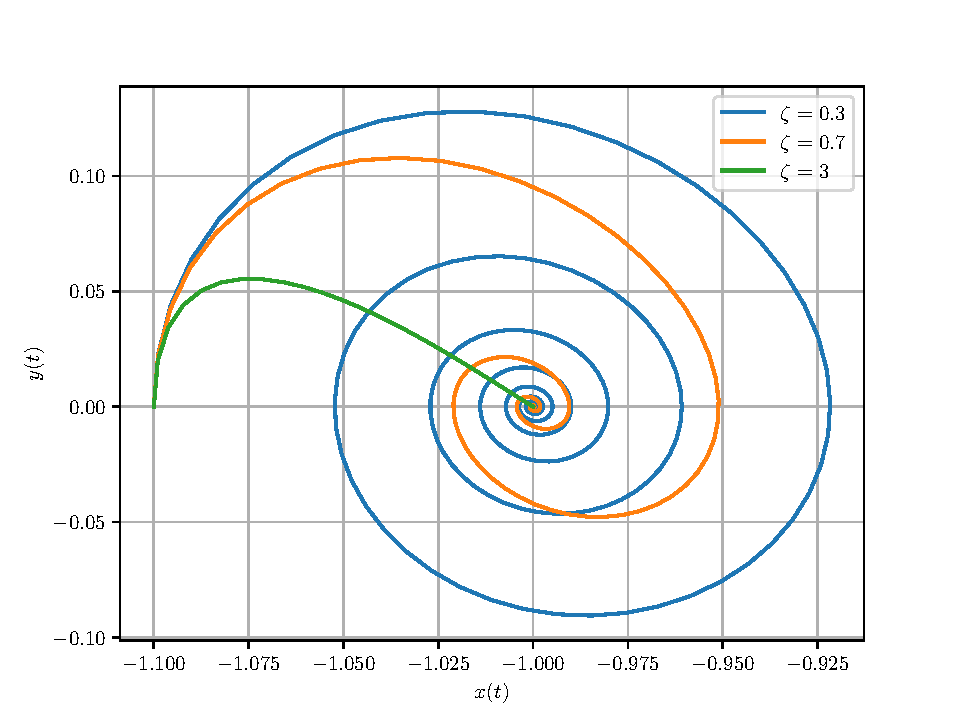
\includegraphics[width=0.9\textwidth]{figures/ex2_attractors.pdf}
        \caption{\gr{Περιοχές έλξης για διάφορα \( \zeta \).}}
        \label{fig:ex2_attractors}
    \end{figure}

    Παρακάτω παρουσιάζονται τα πορτρέτα κίνησης για μικρή απόσβεση,
    \( \zeta = 0.3 \) και μεγάλη \( \zeta = 0.7 \), και το πορτρέτο κίνησης
    για τις δύο τιμές του \( \zeta \).
    \begin{figure}[h]
        \centering
        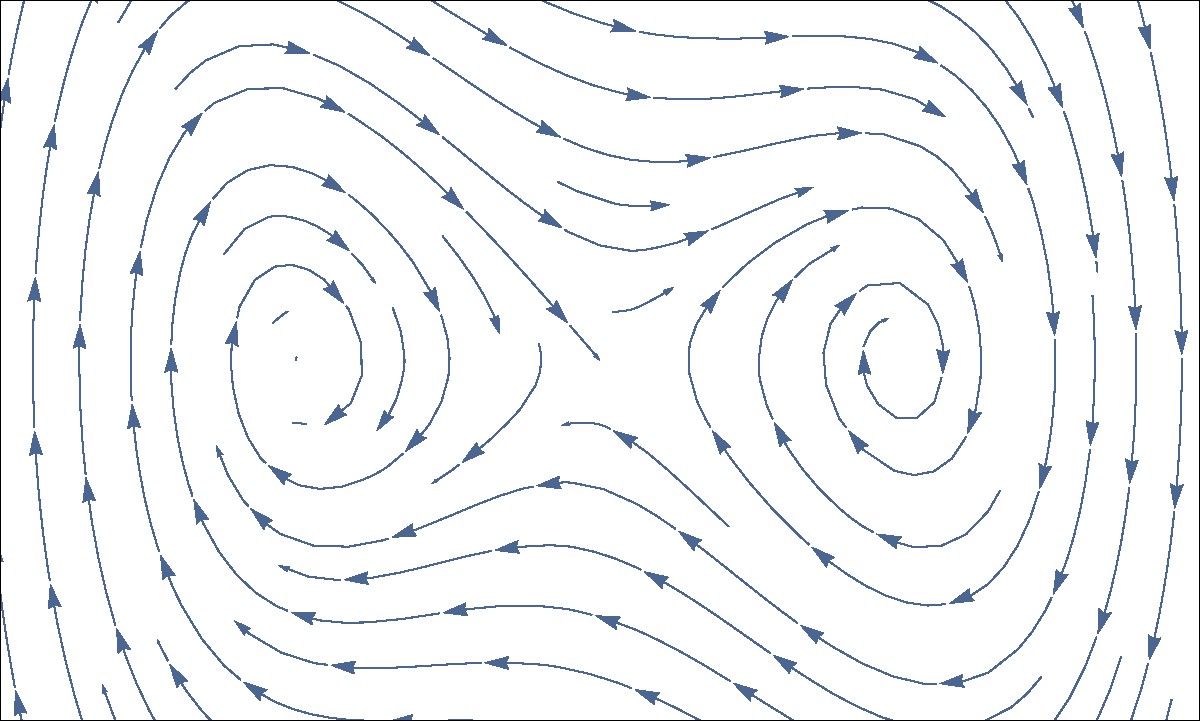
\includegraphics[width=0.8\textwidth]{figures/ex2_dampedDuffing03Vec.pdf}
        \caption{\gr{Πορτρέτο κίνησης ταλαντωτή \tl{Duffing} με απόσβεση,
        \(\zeta = 0.3\).}}
        \label{fig:ex2_dampedDuffing03Vec}
    \end{figure}
    Στο σχήμα~\ref{fig:ex2_dampedDuffing0307Vec}, με το μπλε χρώμα είναι το πεδίο
    για \( \zeta = 0.3 \) και με το καφέ χρώμα το πεδίο για
    \( \zeta = 0.7 \). Από το σχήμα αυτό, αλλά και από το
    σχήμα~\ref{fig:ex2_attractors} είναι φανερό, ότι για μικρό \( \zeta \)
    έχουμε μεγαλύτερες ταλαντώσεις, όπως ήταν αναμενόμενο. Επίσης, από τα διαγράμματα
    αυτά και μόνο είναι φανερό ότι η μεγάλη απόσβεση μας πηγαίνει στα σημεία ισορροπίας
    ταχύτερα. Για μεγαλύτερη έμφαση παρουσιάζεται στο
    σχήμα~\ref{fig:ex2_dampedDuffing} η χρονική απόκριση των μεταβλητών για
    αποσβέσεις \( \zeta = 0.3 \) και \( \zeta = 0.7 \) αλλά και επίσης για
    απόσβεση \( \zeta = 2\sqrt{2} \) έτσι ώστε να φανεί η διαφορετική μορφή σύγκλισης.
    \begin{figure}[h!]
        \centering
        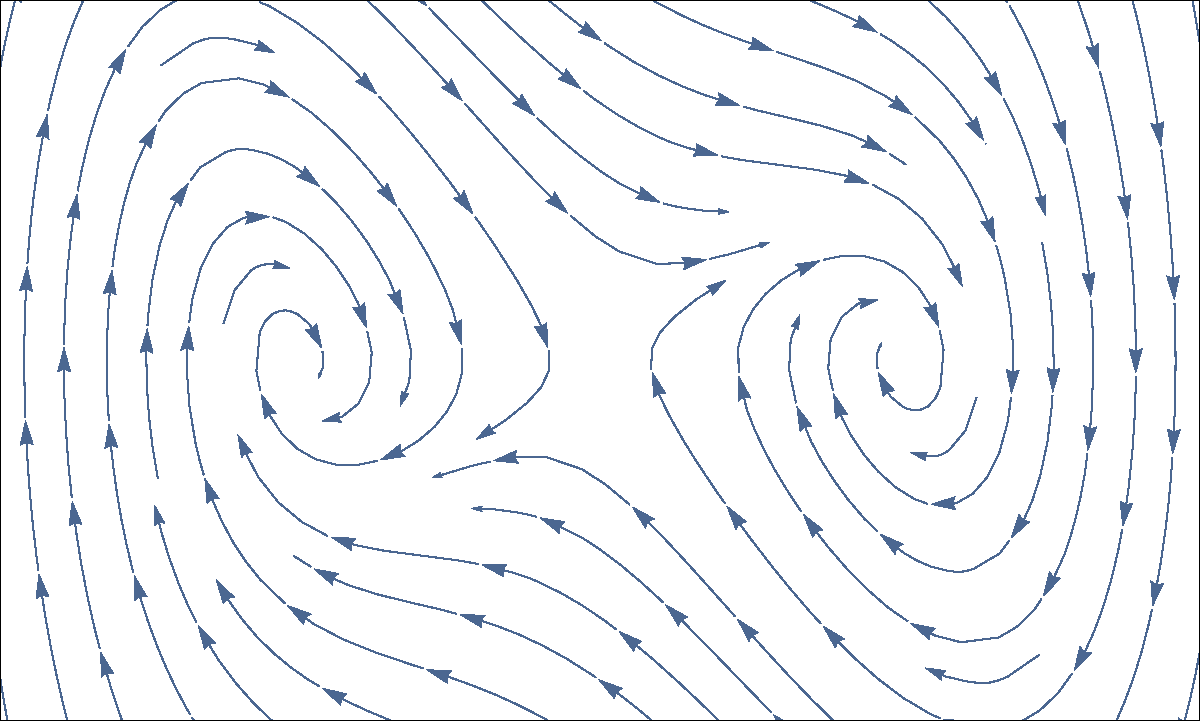
\includegraphics[width=0.8\textwidth]{figures/ex2_dampedDuffing07Vec.pdf}
        \caption{\gr{Πορτρέτο κίνησης ταλαντωτή \tl{Duffing} με απόσβεση,
        \(\zeta = 0.7\).}}
        \label{fig:ex2_dampedDuffing07Vec}
    \end{figure}
    \begin{figure}[h!]
        \centering
        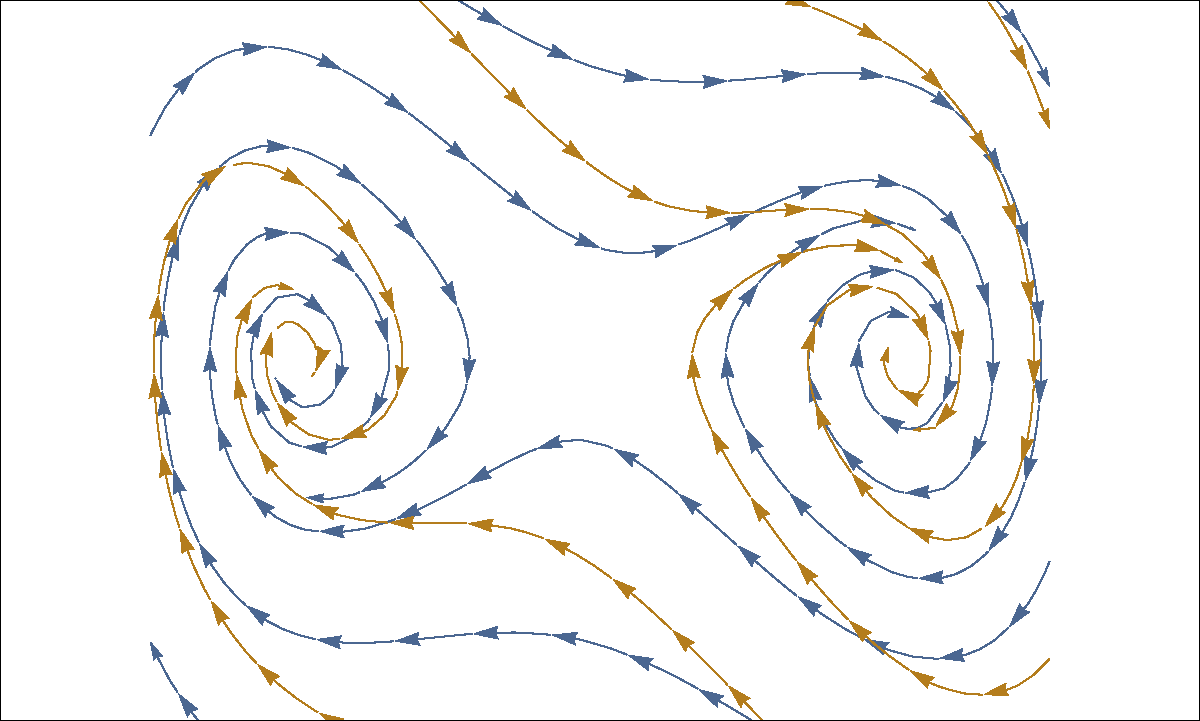
\includegraphics[width=0.8\textwidth]{figures/ex2_dampedDuffing0307Vec.pdf}
        \caption{\gr{Πορτρέτο κίνησης ταλαντωτή \tl{Duffing}
                για \( \zeta = 0.3 \) (μπλε χρώμα) και για \( \zeta = 0.7 \) (καφέ
        χρώμα).}}
        \label{fig:ex2_dampedDuffing0307Vec}
    \end{figure}
    \begin{figure}[h!]
        \centering
        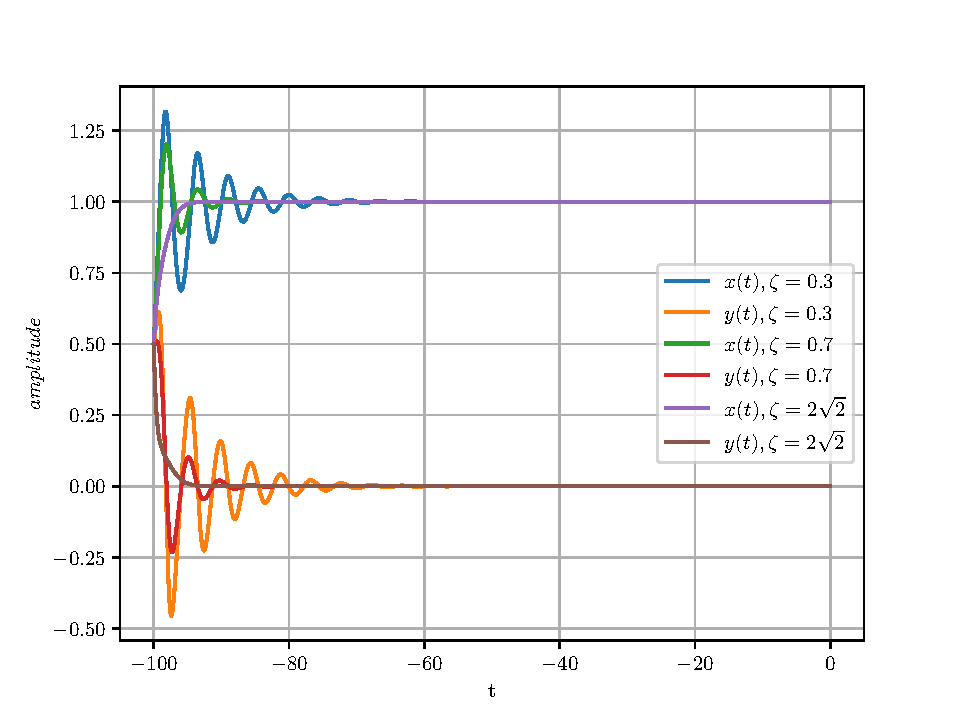
\includegraphics[width=0.9\textwidth]{figures/ex2_dampedDuffing.pdf}
        \caption{\gr{Απόκριση ταλαντωτή \tl{Duffing} για διάφορα \( \zeta \).}}
        \label{fig:ex2_dampedDuffing}
    \end{figure}
\end{solution}
